\input{../header}
\rhead{Your name: \rule{8cm}{0.15mm}}

\begin{document}
%
\section{Learning target AD2, version 1}

Part of the graph of this function $f(x)$ has been erased. 
We'll use linear approximation to recover the values.

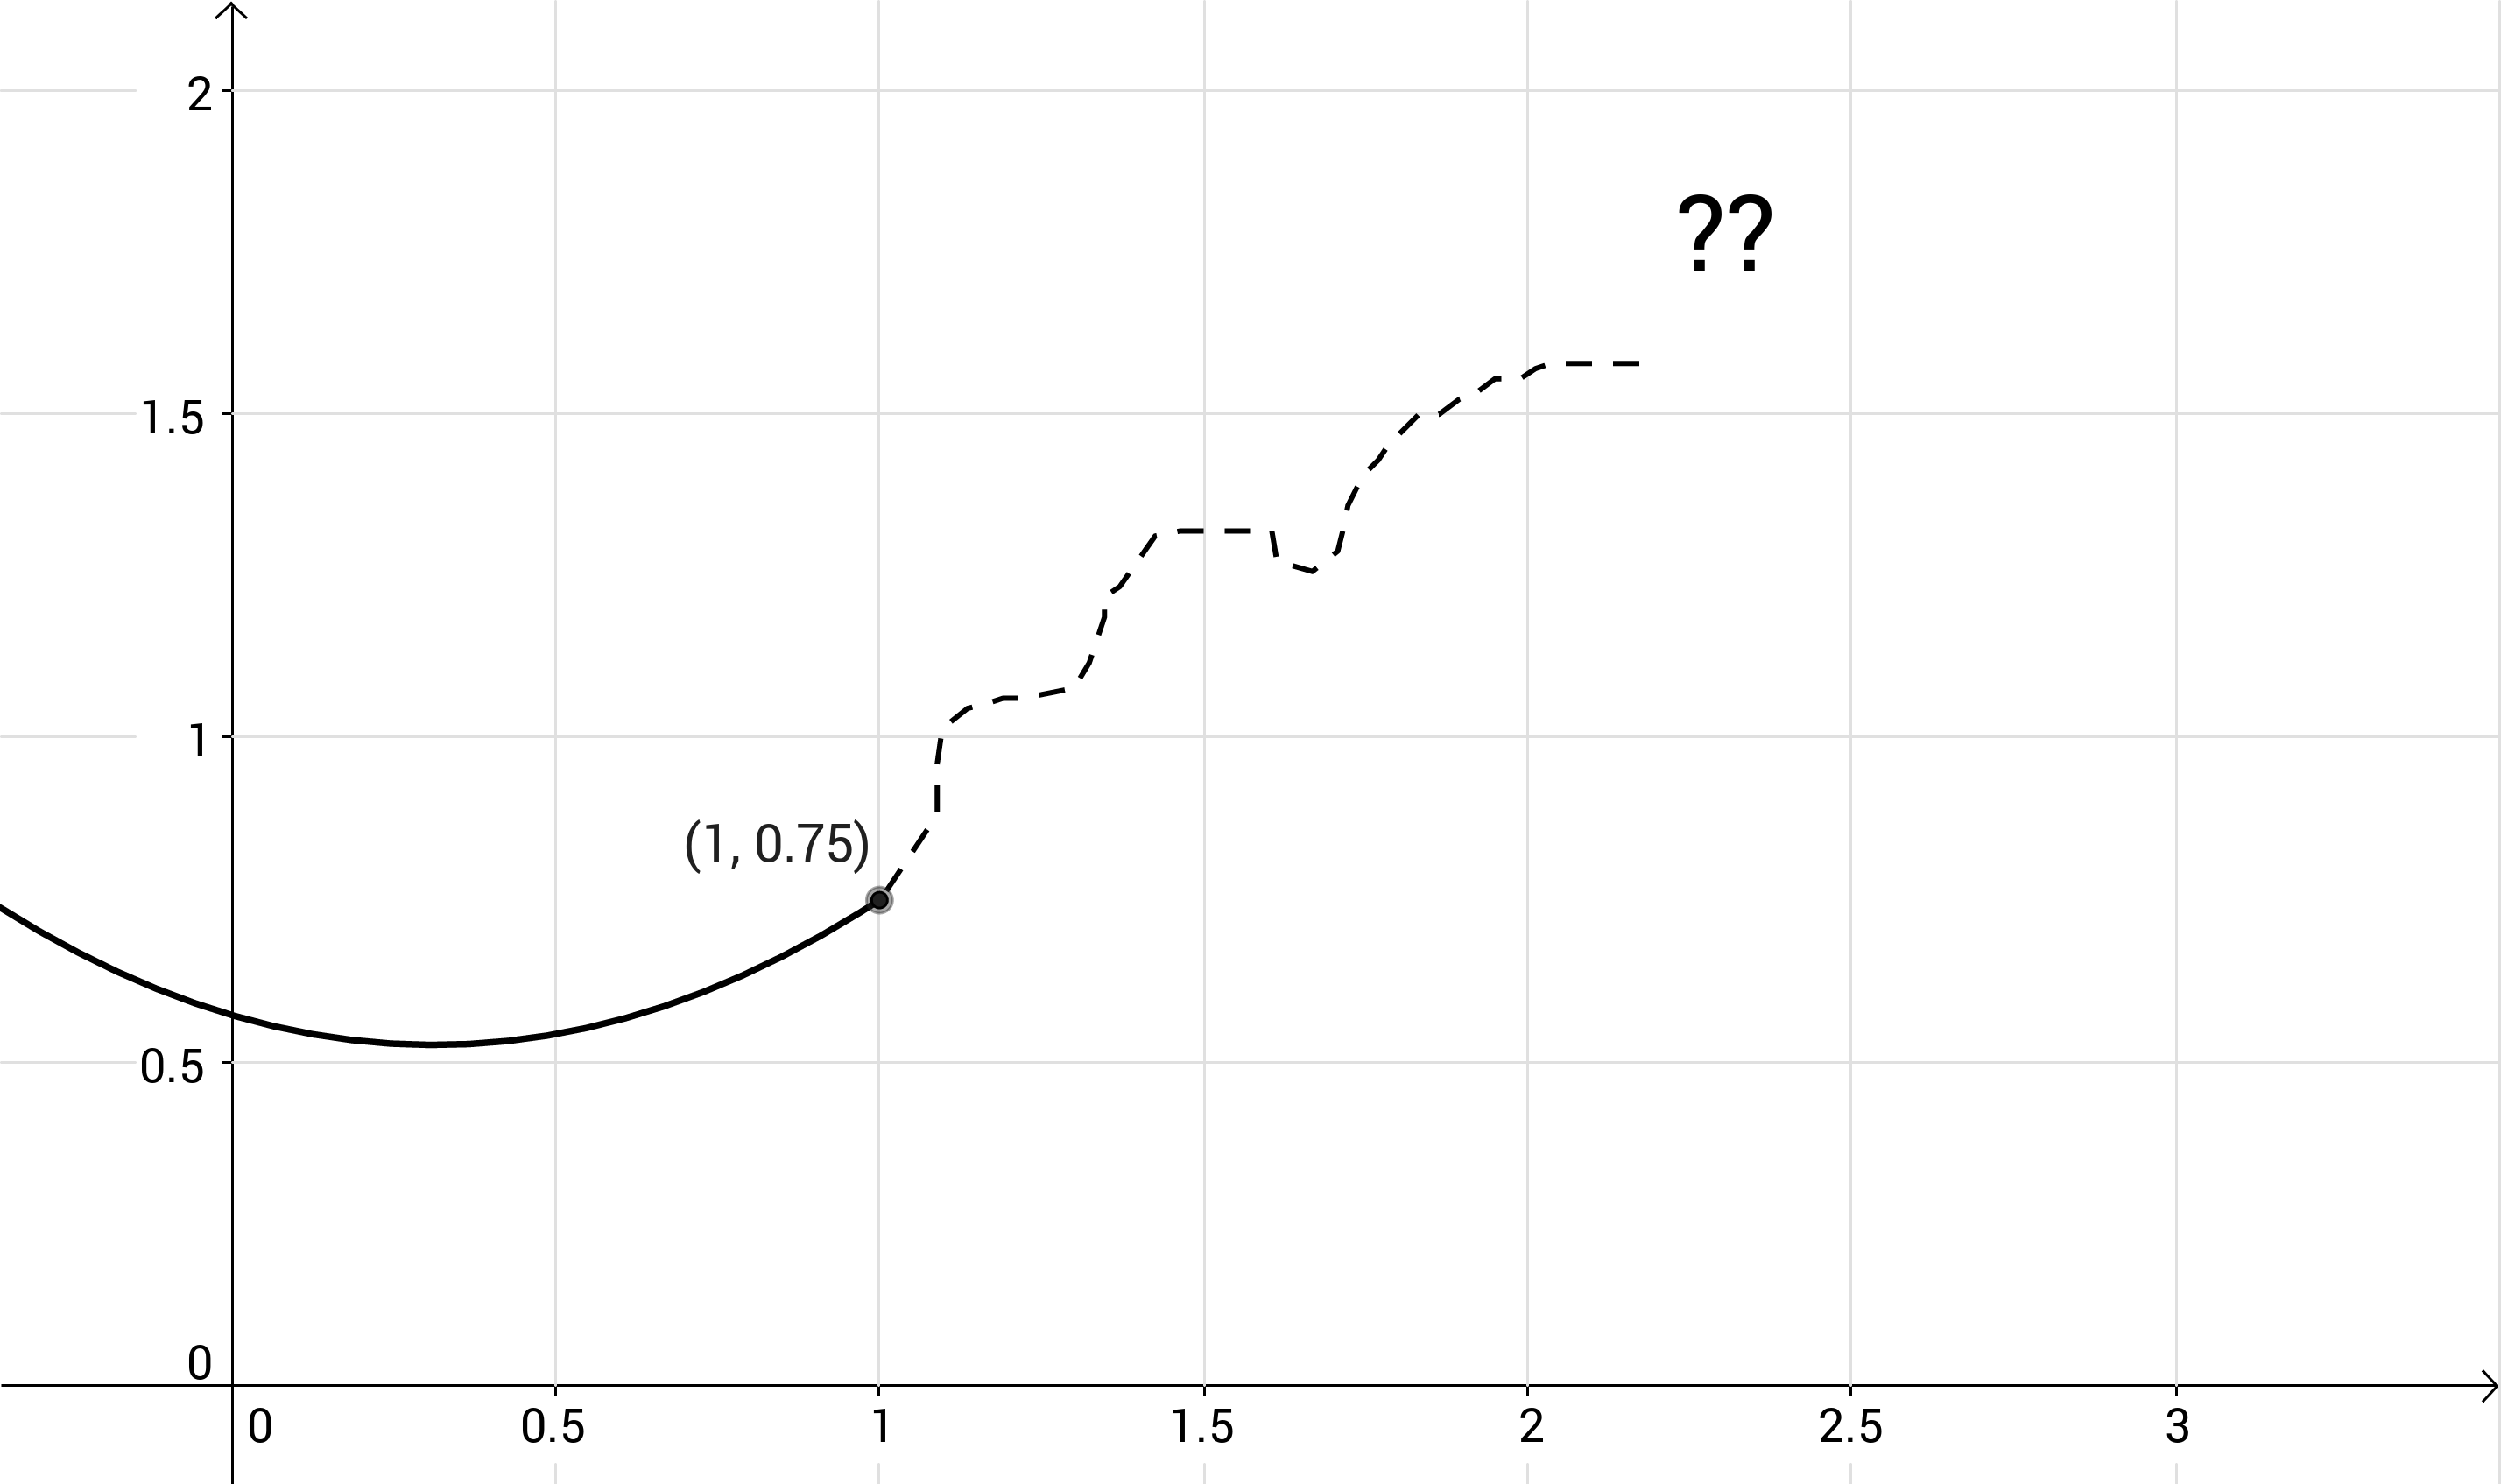
\includegraphics[width=\textwidth]{../images/linapprox.png}

\begin{enumerate}[(a)]
\item Draw the tangent line to this function at $x = 1$.
\item Suppose we know that $f'(1) = 0.65$. Use point-slope form to write down an equation for $L(x)$, the tangent line to this function at $x=1$.
\vfill
\item Use your equation for $L(x)$ to estimate $f(1.4)$.
\vfill
\item Do you think it is more likely that this is an 
overestimate or an underestimate? How come?
\vfill
\end{enumerate}
\end{document}